% !TEX root = ../thesis.tex
\section{Figures}
	\label{sec:typesetting_figures}

In this template figures are numbered starting with the current chapter number followed by a figure number that resets to 1 each new chapter.
As you can see below, the first figure is labelled \cref{fig:dragon} because we are in \cref{chap:typesetting}.
	
Figures in \LaTeX{} are defined using a \lstinline|\begin{figure}...\end{figure}| environment and often immediately begin rendering in centre aligned mode by calling \lstinline|\centering|.
\Cref{lst:latex_figure} below shows the \LaTeX{} code used to typeset \cref{fig:dragon}. \Cref{fig:example_2x1,fig:example_2x2} are defined similarly and make additional use of the \lstinline|\subfloat| command to position multiple images within a single figure environment, each with their own automatically incremented labels and individual captions.

	\lstinputlisting[label={lst:latex_figure}, caption={An example \LaTeX{} excerpt demonstrating how to typeset \cref{fig:dragon} with a simple caption.}]{./listings/example_figure.tex}


	\subsection{Consistent presentation throughout the document}

Figures work best in a document when you use a consistent style for formatting and captioning them, and make sure that figures always actively support the content of the main text. 


	\subsection{Justified use of space in the document}

All figures must be referred to directly in the main text of the document and discussed with meaningful and in depth critical analysis.
If you don't need to use the figure to leverage and support your discussion then it is just taking up space and padding out the document.
For example, you can use a command like \lstinline|\cref{fig:dragon}| to automatically get the figure label for \cref{fig:dragon}. 	

		% !TEX root = ../thesis.tex
% [H] means put the figure HERE, directly when you input this code.
% Remove this to let LaTeX place the figure where it decides is best
\begin{figure}[H]
	\centering

% We set the width of the figure based on the width of one line of text on the page. 
% The value can be tuned to any value in [0.0, 1.0] to scale the image while 
% maintaining its aspect ratio.
	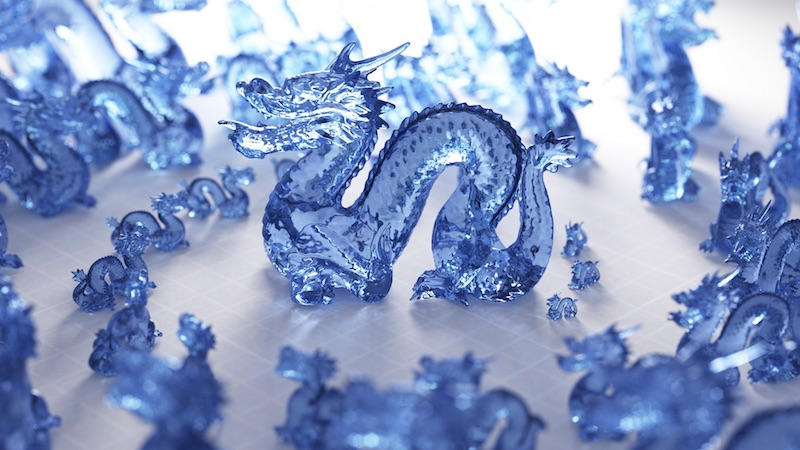
\includegraphics[width=1.0\textwidth]{dragon.jpg}
	
% Caption is defined with a short and long version. The short version is shown in the 
% List of Figures section, and the long version is used directly with the figure. 		
	\caption[An image of many glass dragons being used to demonstrate typesetting a figure.]{
A good caption should be sufficient enough to put the figure in context even if the reader has randomly flicked to the current page and looked only at the figure in isolation.
All figures should also be referred to directly within the main text of your document.
You can use the \LaTeX{} \texttt{\(\backslash\)cref\{key\}} command to insert the correct figure number when you refer to it in the main text.
By the very logic of this caption, this is a very poor caption because we still don't know why on earth is there an picture of glass dragons here.
Image of glass dragons rendered using Path Tracing \cite{whittle15_dragons}.
	
% Figure labels should be defined at the end of the caption to ensure proper numbering.
	\label{fig:dragon}
	}
	
\end{figure}


	\subsection{Placement that supports and enhances the flow of the document}

All figures shown in your document should be displayed in relevant locations.
The definition of ``relevant'' can be a matter of preference, however.
\LaTeX{} defaults to balancing figure and text placement, often preferring, \eg the top or bottom of a nearby page, rather than the location at which you insert a figure command.
This style is often preferable, especially for two-column documents, but can sometimes break up the flow of a single column dissertation-like document, for which it is can sometimes be better to reference figures just after they have been alluded to in the main text.
The examples in this document control figure placement by forcing them to appear exactly where referenced using the \lstinline|[H]| parameter.
See the example figures and online resources for more information about figure placement options.


	\subsection{Avoid directly importing other peoples images}

You should avoid using other people's figures whenever possible, and instead create your own figures for visualising the specific methods and data you are working with in a way directly relevant to your project. 


	\subsection{Format sub-figures in \LaTeX{}, not in the image itself}

Construct sub-figures from multiple image files in \LaTeX{} not in the image file itself.
This allows you to tweak the positioning and layout without having to modify the images.
It also allows for automatic formatting and numbering of captions and sub-captions. \Cref{fig:example_2x1,fig:example_2x2} show examples of side-by-side and quad layouts respectively.
		
		% !TEX root = ../thesis.tex
% [H] means put the figure HERE, directly when you input this code.
% Remove this to let LaTeX place the figure where it decides is best
\begin{figure}[H]
	\centering
	
% We use a figure width of 48.5% of the width of one line of text on 
% the page so there is some space between the images.
	\subfloat[Left image sub-caption.]{
		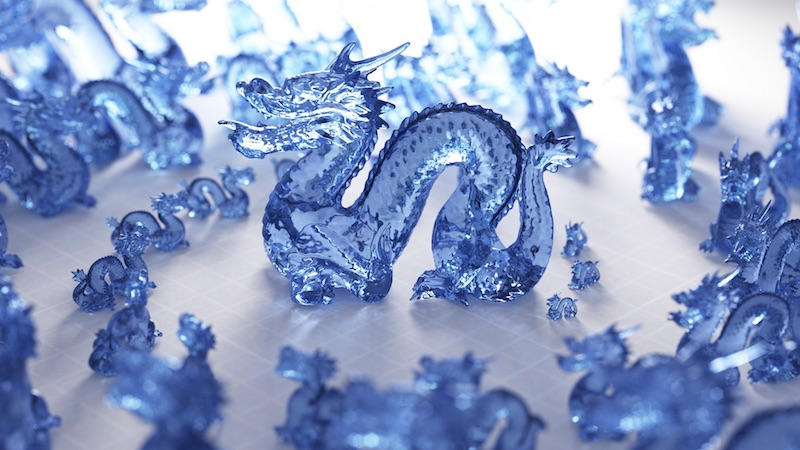
\includegraphics[width=0.485\textwidth]{dragon.jpg}\label{fig:example_2x1_a}
	}\hfill % Spacing between sub-figures displayed next to each other.
	\subfloat[Right image sub-caption.]{
		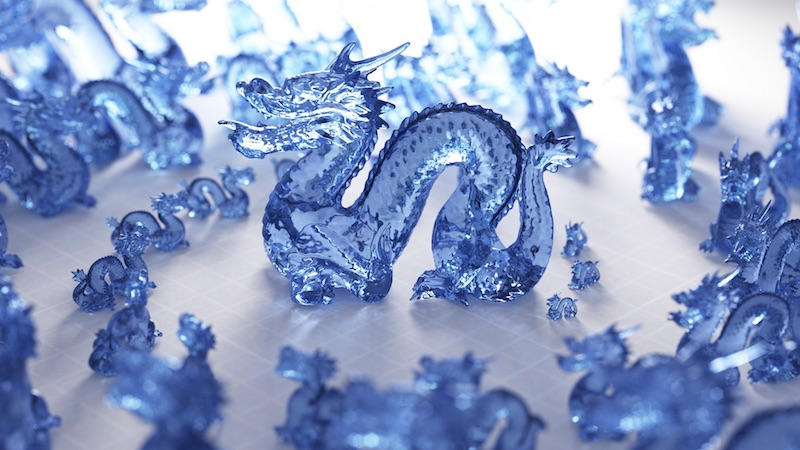
\includegraphics[width=0.485\textwidth]{dragon.jpg}\label{fig:example_2x1_b}
	}\\ % New line before caption.

% Caption is defined with a short and long version. The short version is shown in the 
% List of Figures section, and the long version is used directly with the figure. 	
	\caption[A demonstration of a 2x1 sub-figure layout.]{
Construct sub-figures from multiple image files in \LaTeX{} rather than in the image file itself.
This allows you to tweak the positioning and layout without having to modify the images.
It also allows for automatic formatting and numbering of captions and sub-captions.
Image of glass dragons rendered using Path Tracing \cite{whittle15_dragons}.
	
% Figure labels should be defined at the end of the caption to ensure proper numbering.
	\label{fig:example_2x1}
	}
	
\end{figure}
		
		% !TEX root = ../thesis.tex
% [H] means put the figure HERE, directly when you input this code.
% Remove this to let LaTeX place the figure where it decides is best
\begin{figure}[H]
	\centering
	
% We use a figure width of 48.5% of the width of one line of text on 
% the page so there is some space between the images.
	\subfloat[Top-Left image sub-caption.]{
		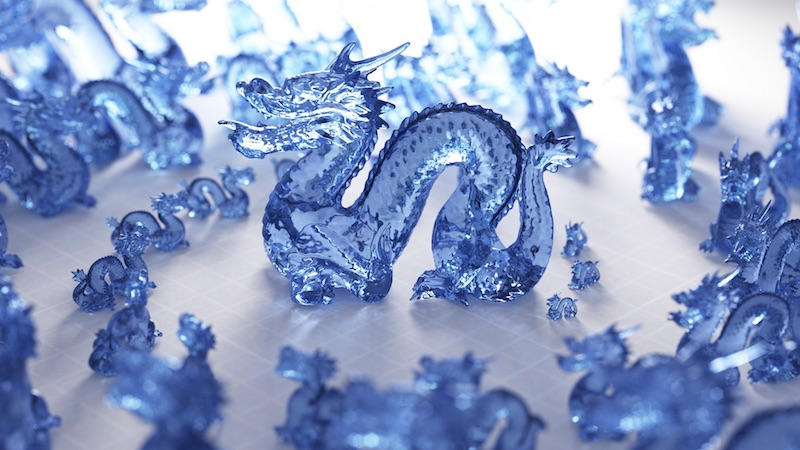
\includegraphics[width=0.485\textwidth]{dragon.jpg}\label{fig:example_2x2_a}
	}\hfill % Spacing between sub-figures displayed next to each other.
	\subfloat[Top-Right image sub-caption.]{
		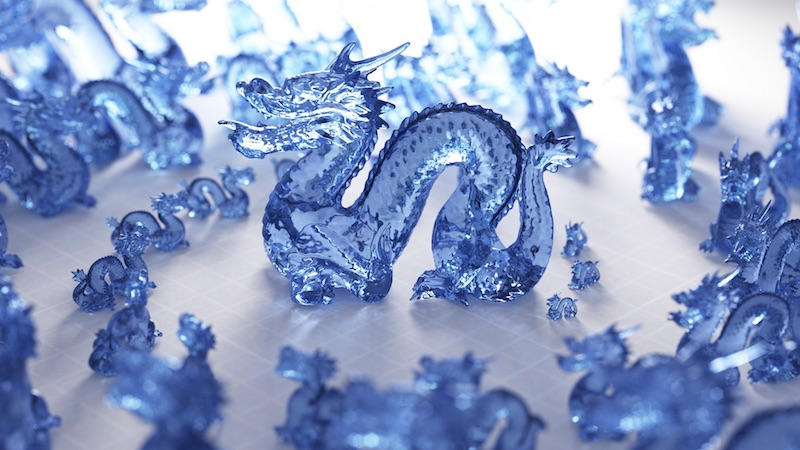
\includegraphics[width=0.485\textwidth]{dragon.jpg}\label{fig:example_2x2_b}
	}\\ % New line before caption.
	\subfloat[Bottom-Left image sub-caption.]{
		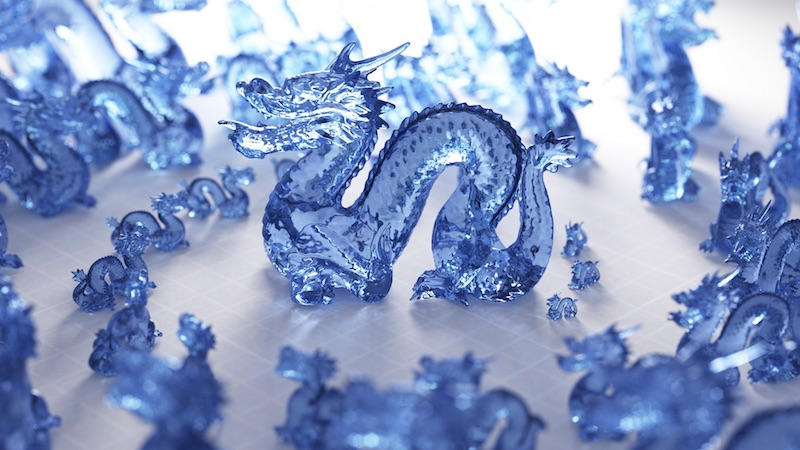
\includegraphics[width=0.485\textwidth]{dragon.jpg}\label{fig:example_2x2_c}
	}\hfill % Spacing between sub-figures displayed next to each other.
	\subfloat[Bottom-Right image sub-caption.]{
		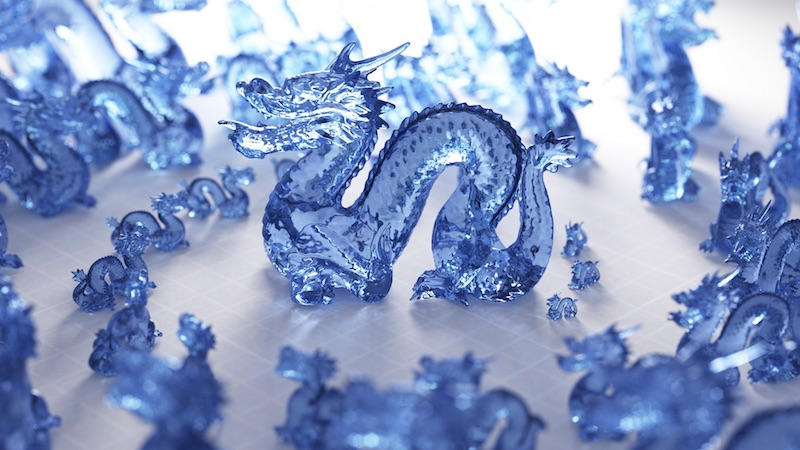
\includegraphics[width=0.485\textwidth]{dragon.jpg}\label{fig:example_2x2_d}
	}\\ % New line before caption.
		
% Caption is defined with a short and long version. The short version is shown in the 
% List of Figures section, and the long version is used directly with the figure. 	
	\caption[A demonstration of a 2x2 sub-figure layout.]{
A demonstration of a 2x2 sub-figure layout.
Between (a)--(b) and (c)--(d) we use \texttt{\(\backslash\)hfill} and between (b)--(c) we use a new line.
Image of glass dragons rendered using Path Tracing \cite{whittle15_dragons}.
	
% Figure labels should be defined at the end of the caption to ensure proper numbering.
	\label{fig:example_2x2}
	}
	
\end{figure}


	\subsection{Robust captions that can stand in isolation}

Figures need to be captioned such that they can be viewed in isolation and still be meaningful to the viewer.
There will likely be some duplication of information that is written in the main text, but this is intended. 


	\subsection{Proper attribution and citation of images}
		\label{sec:typesetting_figures_citation}
		
If an image does not belong to you it \textbf{must} be cited directly in the figure caption. \textbf{It is not correct to put a URL in the figure caption directly.}
A URL in isolation is not an accurate or reliable way of directing a future reader to the exact content you are referencing.
Instead, make a new entry in your \lstinline|citations.bib| file and then reference that citation in the caption using the \lstinline|\cite{key}| command.
\Cref{fig:dragon,fig:example_2x1,fig:example_2x2} each include a statement in the caption stating ``Image of glass dragons rendered using Path Tracing \cite{whittle15_dragons}.''.
When adding the Bib\TeX{} entry, try to find the proper information about the original author and source document to strengthen the citation in case the URL changes.
